%!TEX root = ../PhDthesis.tex
\chapter{Spatially calibrating models of primary visual cortex}

One of the major obstacles in modern neuroscience is integrating the
vast amount of experimental data that has been generated, highlighting
where different sources of evidence is and is not in agreement and
offering testable hypothesis to resolve such discrepancies. The
primary visual cortex is one of the most well studied areas in the
mammalian brain and we have previously seen that it has been
extensively explored at varying levels of description, from
development, circuits and anatomy to surround modulation, behavioural
studies and theoretical models of computation.

In order to provide a better account on how all this information fits
together in a generalized model describing the organization and
computations performed by the cortex, a unified reference frame
regarding the various spatial scales and their origins is desparately
needed. A careful read of the literature highlights just how dependent
various effects are on the spatial scales involved. Here we will
present a model that takes these various levels of evidence into
account to allow comparing whether using known anatomical properties
we can predict the known response properties of the cortex after
development. This will allow bridging between known measurements of
anatomy and circuitry and electrophysiological or even behavioral
experiments performed on visual cortex.

So far only very few attempts have been made at developing models that
take into account the various spatial properties that have been
described in the literature ranging from anatomy to
electrophysiological measurements. In particular to begin making sense
of the surround modulation literature, which is highly dependent on
the precise choice of stimulation protocol, it is essential to take
into the various spatial scales involved. Therefore this chapter will
demonstrate how existing models of cortical development, specifically
the Gain Control Adapation Lateral model (GCAL) \citep{Stevens2013}
can be calibrated to match known measurements of spatial extents more
closely in a new S-patially CAL-ibrated (SCAL) model.

The analysis will focus on various experimental assessments of the
spatial properties of the visual pathway and describe how we can use
these to build a model that achieves a high-level of consistency with
experimental results across a wide range of measures. Specifically, we
will attempt to calibrate the model with experimental measurements in
the parafoveal regions of the visual system of macaque. The macaque
has long been a experimental model for in visual neuroscience and the
literature surrounding contextual modulation in particular.

Once we have collected the data we will provide a full
characterization of the spatial response properties, receptive fields
and synaptic weights in the model confirming they closely match
experimental data. At the same time we will outline in which ways the
model falls short and discuss some ways in which these shortcomings
might be remedied.

\section{Methods}

In this chapter we first introduce the developmental models of the
primary visual cortex the more complex models are based on. We begin
by outlining the equations and mechanisms underpinning these models
and then describe various analyses we can apply to these models to
replicate experimental protocols and compare the model against
experimental results.

\subsection{A spatially calibrated model of cortical development} 

The GCAL model put forth in \cite{Stevens2013} will serve as the
starting point for the models in this thesis. As discussed previously
(see \ref{devmodels}), it provides the first model that develops
robust and stable orientation maps independent of visual contrast and
for a wide range of training inputs. In this section we describe the
equations governing this model, how it is structured and will
highlight the modifications that were made to achieve a more
consistent spatial calibration.

\subsubsection{Architecture}

The architecture of this family of models builds on two main concepts,
the idea of 2D sheets of firing-rate point neurons and projections
between them, representing the synaptic connections between the
neurons. All models we will introduce share the same basic
organization at the retinal and lateral geniculate nucleus level, but
will introduce increasingly complex models of the interactions in the
primary visual cortex. In Figure \ref{LGNDiagram} you can see the
organization of the retinal and lateral geniculate nucleus ON and OFF
sheets.

The model operates by presenting patterns on the retinal sheet, which
then get filtered through difference-of-gaussian connection fields,
which give rise to the response the ON and OFF sheets. There a lateral
gain control projection applies some pooling normalization to the
response. This early stage of processing represents a crude model of
retinal ganglion and LGN function and provides the input to the
various cortical models introduced here.

The architecture of the retinal ganglion cell and lateral geniculate
nucleus layers will remain unchanged in the model. Note that the
diagram already specifies the final spatial scales used in this model,
while this section will focus on determining a consistent set of
parameters for the model.

\begin{figure}
	\centering
        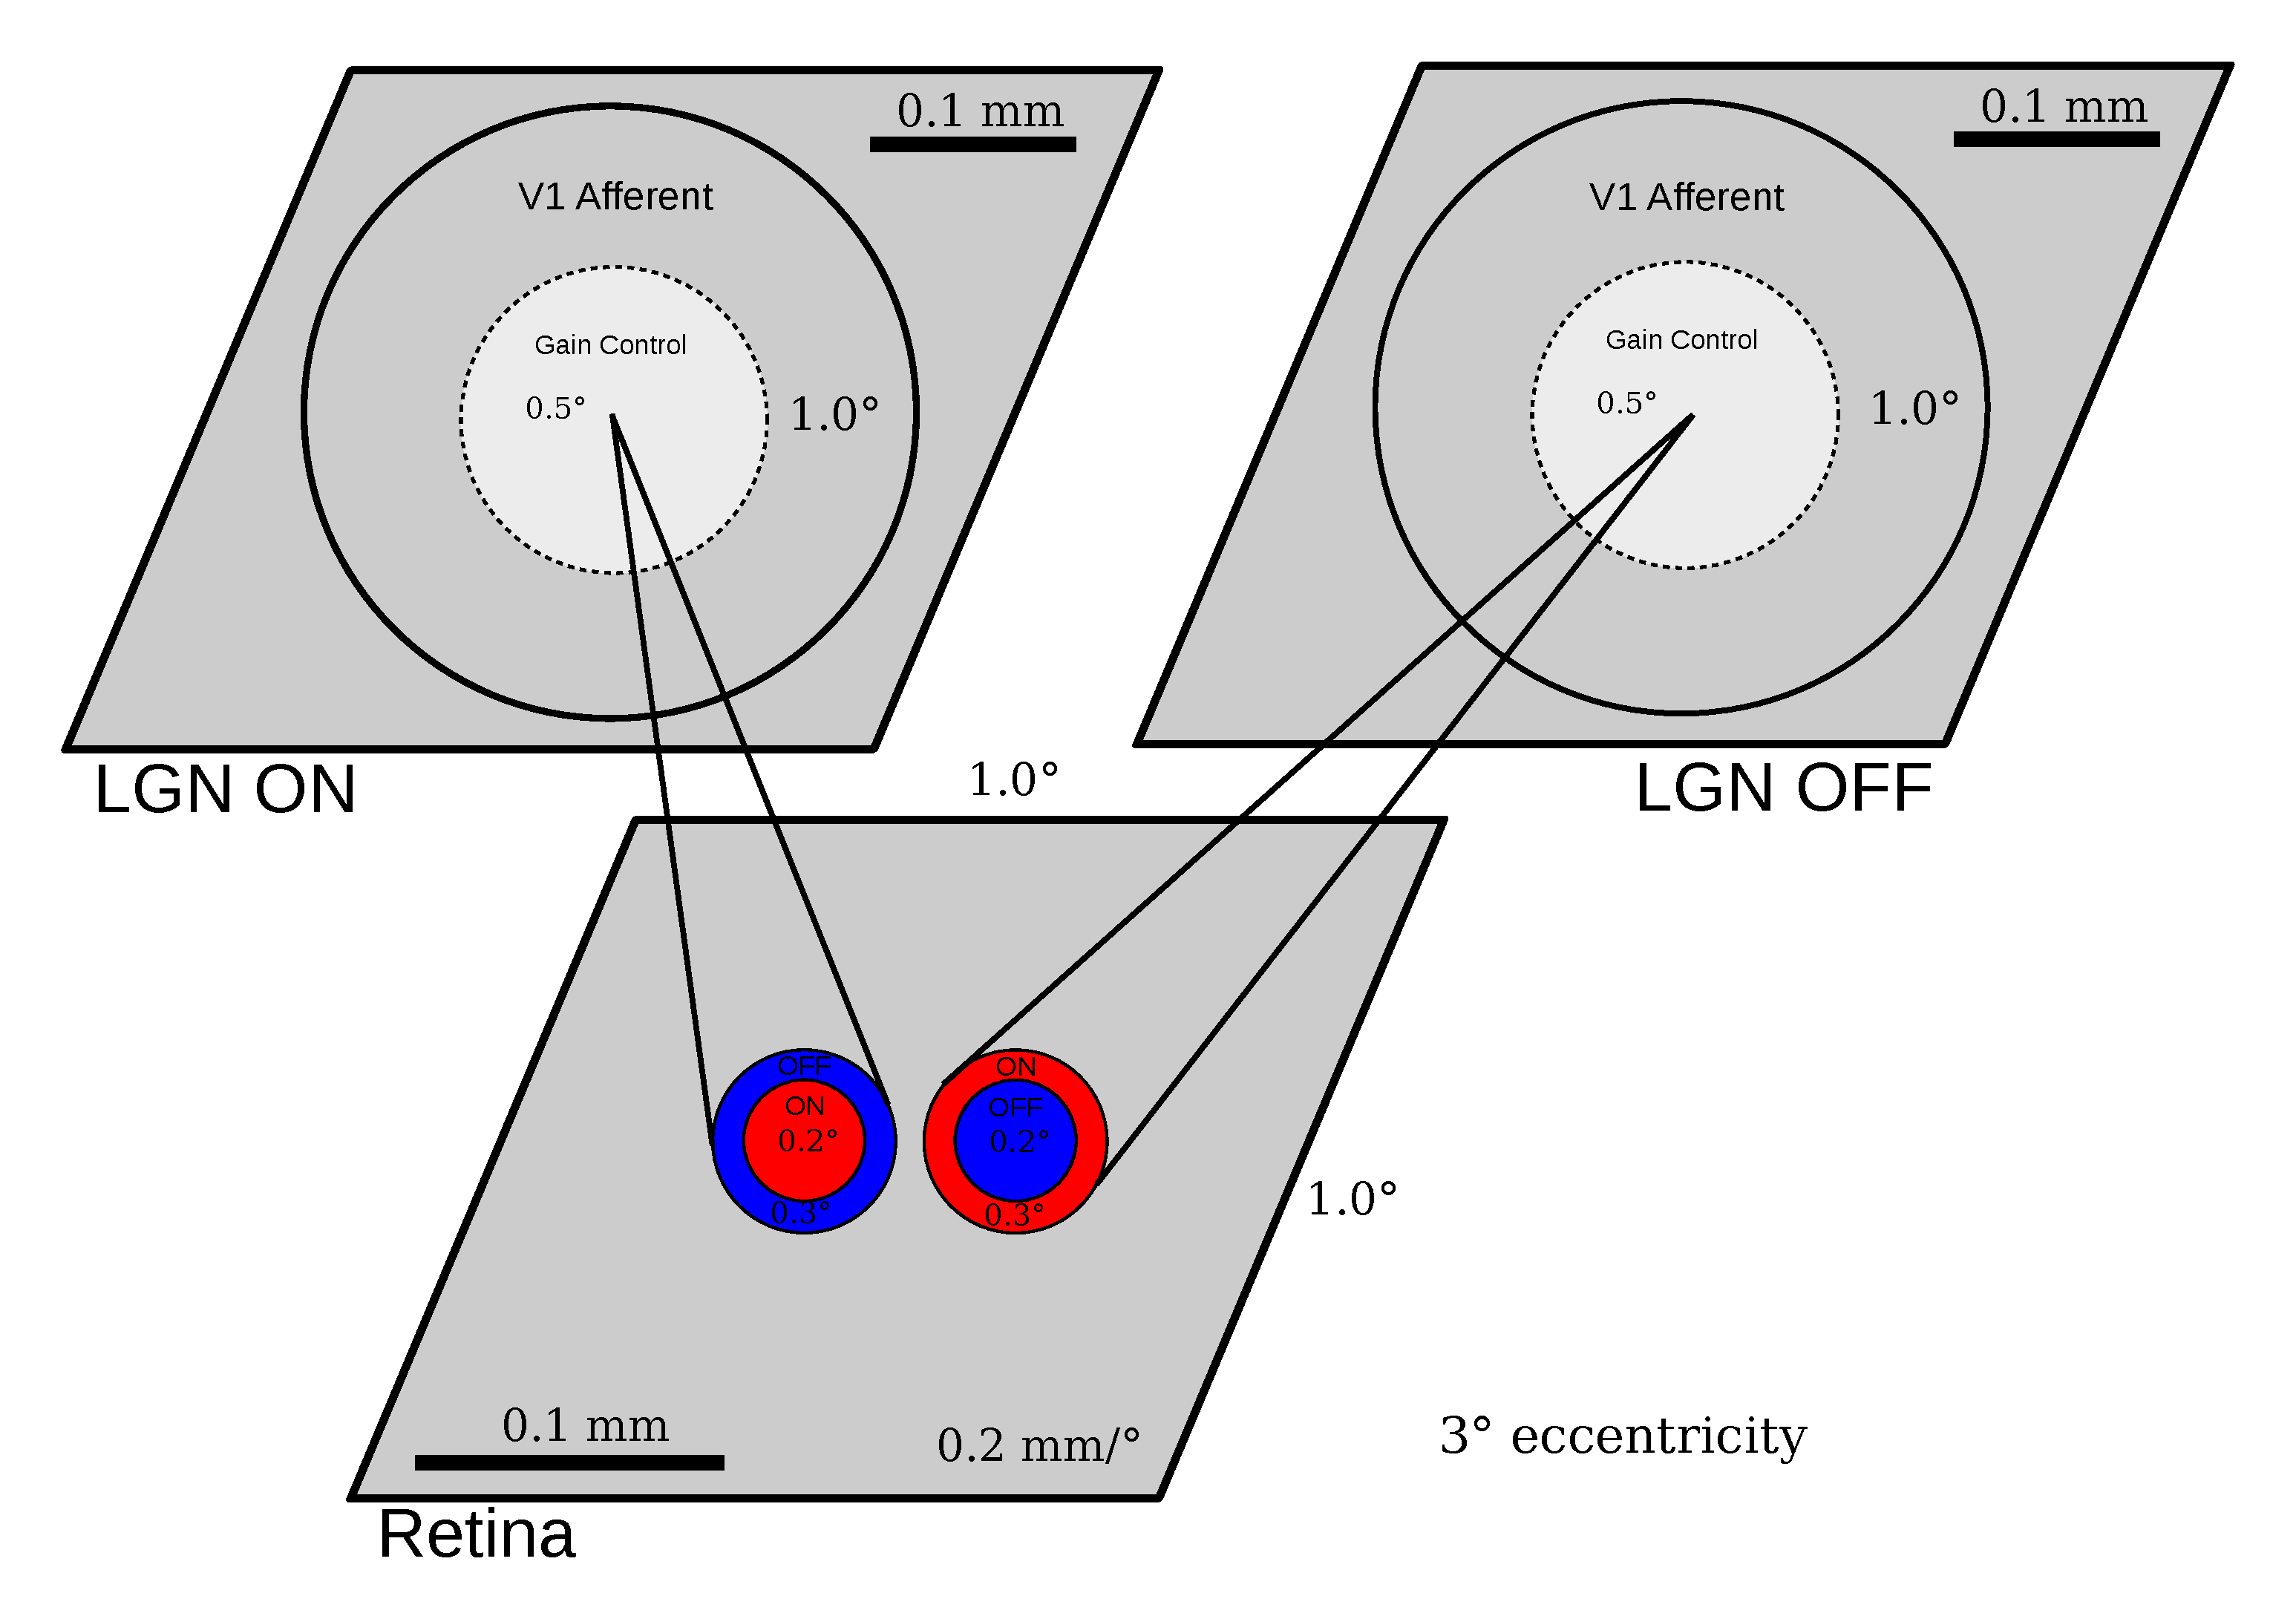
\includegraphics[width=1.0\textwidth]{LGN_Diagram.pdf}
	\caption{Diagram of the SCAL-LGN stage of the model showing
          the spatial scales of the various excitatory (red) and
          inhibitory (blue) connections. Satured colors indicate the
          kernel radii, while lightly shaded regions indicate kernel
          cut-off extents.}
	\label{LGNDiagram}
\end{figure}

\subsubsection{Input patterns}

The organization of the SOM based developmental models of the cortex,
is determined by a complex interplay between the model and the input
patterns it is trained on. Just as in the developing brain connections
are formed depending on the statistics of the sensory experience of
the strongly influencing the spatial organization of the model. In
order to accurately assess how the models respond to and self-organize
in different visual environments we will use three different visual
stimuli to present to the model.

The simplest pattern used as the baseline for most measurements will
be simply elongated Gaussian patterns matching the length of the
integrative area of a V1 neuron and with a spatial frequency that
would allow three distinct lobes to form within this area. The
training patterns are given by:

\begin{equation}
  exp(-x^2/(2*\sigma_x^2) - y^2/(2*\sigma_y^2)
\label{eqn:gausspattern}
\end{equation}

Additionally two image datasets will be employed one taken from a
database of natural images and the other recorded from within the
rearing environment of ferrets in a laboratory, which is dominated by
the long co-linear statistics of the cage bars. These datasets will
allow us to explore the effect of the natural image statistics on the
organization of the models and confirm robustness against a wide range
of visual input.

\subsubsection{Activation}

All the models operate by presenting a new retinal input at each
iteration updating the activation of each unit in each sheet. The
neurons in the sheets are firing-rate point neurons, with the main
state being a floating point activation value.  For all models, the
activation level $\eta$ for a unit at position $j$ in an ON/OFF sheet
O at time $t+\delta t$ is defined as:

\begin{equation}
\eta_{j, O}(t+\delta t)=f\left(\frac{\gamma_{O}\sum_{i\in
    F_{j,P}}\Psi_{i}(t)\omega_{ij}}{k+\gamma_{S}\sum_{i\in
    F_{j,S}}\eta_{i, O}(t)\omega_{ij, S}}\right)
\label{eqn:lgnactivation}
\end{equation}

The constant $\gamma_{O}=14.0$ is an arbitrary multiplier for the
overall strength of connections from the photoreceptor sheet to the
ON/OFF sheets, chosen to give typical activations in the range 0.0 to
1.0, while $\gamma_{S}$ is the strength of the feed-forward
contrast-gain control. $\Psi_{i}$ is the activation of unit $i$ in the
two-dimensional array of neurons on the photoreceptor sheet from which
ON/OFF unit $j$ receives input (its afferent connection field
$F_{j,P}$) and $\eta_{i, O}(t)$ is the activation of other ON/OFF
units on the previous time step (received over the suppressive
connection field $F_{j,S}$). The activation function $f$ is a
half-wave rectifying function that ensures the activation of ON/OFF
units is always positive.

The weights $\omega_{ij}$ represent the fixed connection weights from
photoreceptor $i$ to the ON or OFF unit $j$ defined with a standard
difference-of-Gaussians (DoG) kernel. The connection fields for ON units
have a positive center and negative surround, and vice versa for OFF
units. More precisely, the weight $\omega_{ij}$ from an ON-center cell
at location (0,0) in the ON sheet and a photoreceptor sheet in
location $(x,y)$ on the photoreceptor sheet is given by:

\begin{equation}
\omega_{ij}=\frac{1}{Z_c}\exp{\left(-\frac{x^{2}+y^{2}}{2\sigma_{c}^{2}}\right)}-\frac{1}{Z_s}\exp\left(-\frac{x^{2}+y^{2}}{2\sigma_{s}^{2}}\right)
\label{eqn:DoG}
\end{equation}

The kernel sizes of the central Gaussian $\sigma_{c}$ and surround
mechanism $\sigma_{s}$ are what we will be determinging here. Unlike
simple DoG kernels, the center-surround are jointly normalized to 1.0
using $Z_c$ and $Z_s$. The weights for an OFF-center cell are the
negative of the ON-center weights (i.e., surround minus center). The
center of the connection field of each ON/OFF unit is mapped to the
location in the photoreceptor sheet corresponding to the location of
that unit in sheet coordinates, making the projection retinotopic.

The weights $\omega_{ij, S}$ in the denominator of equation
\ref{eqn:lgnactivation} specify the spatial profile of the lateral
inhibition received from other ON/OFF units when contrast-gain control
is active. The weights of these connections have a fixed, circular
Gaussian profile so that for a neuron located at (0,0) in either the
ON or OFF sheet:
%%
\begin{equation}
\omega_{ij,S}=\frac{1}{Z_S}\exp\left(-\frac{x^{2}+y^{2}}{2\sigma_{S}^{2}}\right)
\label{eqn:gauss}
\end{equation}
%%
where $(x, y)$ is the location of the presynaptic neuron, $\sigma_{S}$
determines the width of the Gaussian, and $Z_S$ is a normalizing
constant that ensures that the total of all the lateral inhibitory
weights $\omega_{ij}$ to neuron $j$ sum to 1.0. This gain-control
projection is activated once per iteration before activity is sent to
the V1 sheet.

\subsubsection{The V1 model}

As we saw above in the LGN section the model described here is heavily
based on the GCAL model \citep{Stevens2013}, however it does differ in
one major respect, it employs divisive rather than subtractive
inhibition.

Each V1 neuron in each model receives connections from three different
connection types or `projections' ($p$), i.e., the afferent projection
from the ON/OFF sheets (both channels concatenated into one input
vector; $p=A$), the recurrent lateral excitatory projection ($p=E$),
and the recurrent lateral inhibitory projection ($p=I$) from other V1
neurons.

The contribution $C_{j,p}$ to the activation of unit $j$ from each
projection type ($p=A,E,I$) is calculated as:
%%
\begin{equation}
C_{j,p}(t+\delta t)=\sum_{i\in F_{j,p}}\eta_{i, p}(t)\omega_{ij,p}
\label{eqn:update}
\end{equation}
%%
where $\eta_{i, p}$ is the activation of unit $i$ taken from the set
of neurons in V1 to which unit $j$ is connected (its connection field
$F_j$) and $w_{ij,p}$ is the connection weight from unit $i$ in V1 to
unit $j$ in V1 for the projection $p$. Afferent activity ($p=A$)
remains constant after the first update from the retina, but the other
contributions change over 16 settling steps, depending on the activity
in V1.

The contributions from all three projections to V1 (afferent
($p_{A}$), excitatory $p_{E}$ and inhibitory $p_{I}$) described above
are combined using equation \ref{eqn:activation1} to calculate the
activation of a neuron $j$ in V1 at time t:
%%
\begin{equation}
\eta_{j,V}(t)=f\left(\frac{\sum_{p=\{E, A\}}\gamma_{p}C_{jp}(t)}{1+\sum_{p=\{I\}}\gamma_{p}C_{jp}(t)}\right)
\label{eqn:activation1}
\end{equation}

The projection strength scaling factors $\gamma$ are defined for each
projection type set to provide a balance between excitation and
inhibition, and between afferent and lateral influences, to provide
robust formation of activity bubbles that allows smooth maps to
form. The function $f$ defines a variable threshold point ($\theta$)
dependent on the average activity of the unit as described in the next
subsection, but in all cases the gain is fixed at unity.

At the end of the 16 settling steps, the settled V1 activation pattern
is deemed to be the V1 response to the presented pattern. At this
point we use the V1 response to update the threshold point ($\theta$)
of V1 neurons (using the adaptation process described below) and to
update the afferent and lateral inhibitory weights via Hebbian
learning. Unlike the regular GCAL model the V1 activity is not reset
to zero instead being allowed to decay until the onset of the next
visual input pattern.

\subsection*{Adaptation}

In order to set the threshold for activation, each neuron unit $j$ in
V1 calculates a smoothed exponential average of its settled activity
patterns ($\overline{\eta_{j}}$):
%%
\begin{equation}
\overline{\eta_{j}}(t)= (1-\beta)\eta_{j}(t) + \beta\overline{\eta_{j}}(t-1)
\label{eqn:averaging}
\end{equation}

The smoothing parameter ($\beta=0.991$) determines the degree of
smoothing in the calculation of the average. $\overline{\eta_{j}}$ is
initialized to the target average V1 unit activity ($\mu$), which for
all simulations is $\overline{\eta_{jA}}(0) = \mu= 0.024$. The
threshold is updated using:
%%
\begin{equation}
\label{eqn:thresholdupdate}%
\theta(t)= \theta(t-1) + \lambda(\overline{\eta_{j}}(t) -\mu)
\end{equation}
%%
where $\lambda=0.01$ is the homeostatic learning rate. The effect of
this scaling mechanism is to bring the average activity of each V1
unit closer to the specified target. If the activity in a V1 unit
moves away from the target during training, the threshold for
activation is thus automatically raised or lowered in order to bring
it closer to the target. Note that an alternative rule with only a
single smoothing parameter (rather than $\beta$ and $\lambda$) could
be formulated, but the rule as presented here makes it simple for the
modeler to set a desired target activity $\mu$.

\subsection*{Learning}

Initial connection field weights are isotropic 2D Gaussians for the
lateral excitatory projection and uniformly random within a Gaussian
envelope for afferent and lateral inhibitory
projections. Specifically, for a neuron located at (0,0):
%%
\begin{equation}
\omega_{ij}=\frac{1}{Z_p}u\exp\left(-\frac{x^{2}+y^{2}}{2\sigma_{p}^{2}}\right)
\label{eqn:gaussrandomweights}
\end{equation}
%%
where $(x, y)$ is the sheet-coordinate location of the presynaptic
neuron, $u=1$ for the lateral excitatory projection ($p=E$) and $u$ is
a scalar value drawn from a uniform random distribution for the
afferent and lateral inhibitory projections ($p=A,I$), $\sigma_{p}$
determines the width of the Gaussian in sheet coordinates
($ \sigma_{A}=0.27, \sigma_{E}=0.025, \sigma_{I}=0.075$), and $Z_p$ is
a constant normalizing term that
ensures that the total of all weights $\omega_{ij}$ to neuron $j$ in
projection $p$ is 1.0.  Weights for
each projection are only defined within a specific maximum circular
radius $r_p$ ($r_{A}=0.27, r_{E}=0.1, r_{I}=0.23$).

In the model, as images are presented to the photoreceptors, V1
afferent connection weights $\omega_{ij,A}$ from the ON/OFF sheets are
adjusted once per iteration (after V1 settling is completed) using a
simple Hebbian learning rule. This rule results in connections that
reflect correlations between the pre-synaptic ON/OFF unit activities
and the post-synaptic V1 response.  Hebbian connection weight
adjustment at each iteration is dependent on the pre-synaptic
activity, the post-synaptic response, and the Hebbian learning rate:
%%
\begin{equation}
\omega_{ij,p}(t)=\frac{\omega_{ij,p}(t-1)+\alpha\eta_{j}\eta_{i}}{\sum_{k}\left(\omega_{kj,p}(t-1)+\alpha\eta_{j}\eta_{k}\right)}
\label{eqn:hebb}
\end{equation}
%%
where for unit $j$, $\alpha$ is the Hebbian learning rate for the
afferent connection field $F_{j}$. Unless it is constrained, Hebbian
learning will lead to ever-increasing (and thus unstable) values of
the weights \citep{Rochester1956}. In all the models the weights are
constrained using divisive post-synaptic weight normalization
(equation \ref{eqn:hebb}), which is a simple and well understood
mechanism. Afferent connection weights from ON and OFF units are
normalized together in the model. We expect that a more biologically
motivated homeostatic mechanism for normalization such as
multiplicative synaptic scaling
\citep{Turrigiano1999,Turrigiano2004,Sullivan2006} or a sliding
threshold for plasticity \citep{Bienenstock1982} would achieve similar
results, but have not tested these.

The learning rates $\alpha$ are defined separately for the afferent,
lateral excitatory and lateral inhibitory projections. The
density-specific value used in the equation above is then calculated
as $\alpha=\frac{\alpha_{A}}{\tau_{A}}$, where $\tau_{A}$ is the
number of connections per connection field in the afferent projection.

\subsection{Analyses}

In order to analyse the spatial organization of the developed model we
borrow from a variety of techniques used to analyse
electrophysiological, optical imaging and anatomical data obtained in
vivo allowing us to compare directly between experimental results and
our model.

\subsubsection{Area summation curves}

The area summation curves were measured in the model by presenting the
model with disks of sine gratings of increasing size and varying phase
and at the optimal spatial frequency of each neuron. The size tuning
curves obtained in this way were then fitted with the integrated
Difference of Gaussian model described by the following equation:

\begin{equation}
R(s) = R_0 + K_e \int \int re^{-\frac{r^2}{a}} \,
\mathrm{d}r\mathrm{d}\theta - K_i \int\int re^{-\frac{r^2}{b}} \,
\mathrm{d}r\mathrm{d}\theta
\label{iDoG}
\end{equation}

\noindent where $R_0$ is the spontaneous response rate, $K_e$ the
excitatory gain, $K_i$ the inhibitory gain, $a$ the excitatory space
constant and $b$ the inhibitory space constant. By separating the
inhibitory and excitatory components in equation \ref{iDoG} and define
them as $R_e$ and $R_i$, we can formulate a subtractive and divisive
version of this equation:

\begin{equation}
R = R_e - R_i
\label{DoGSubstractive}
\end{equation}

\begin{equation}
R = \frac{R_e}{1+R_i}
\label{DoGDivisive}
\end{equation}

Using the estimated spatial constants and gain parameters we can also
calculate the suppression index of each neuron

Unlike in the original experiment we eliminate the $R_0$ and $\beta$
parameters from both models since they represent the baseline activity
and the spiking threshold respectively, which does not apply to a
firing-rate model. After fitting this model we calculate the
mean-squared error (MSE) and the explained variance of the model
($R^2$) to characterize the goodness of fit and compare how well the
two models can capture the data. Furthermore we can determine the
suppression index for the model, which is defined.

\subsubsection{Hypercolumn distance}

One of the major features of the development of the visual cortex in
higher mammals is the organization of neurons into orderly topographic
maps, forming smoothly varying feature preferences across the cortical
surface. In particular the LISSOM family of models has been able to
develop highly realistic orientation maps. These maps have been
studied in detail in various animal species and precise estimates for
their spatial scales are known. \cite{Kaschube2010} were able to
provide a detailed account of the hypercolumn distances in different
species. The hypercolumn distance is defined as the distance on the
cortical surface at which the orientation preference wraps around.

The hypercolumn distance is determined by taking the 2D fast Fourier
transform of the orientation map and collapse the real component to
1D, allowing us to determine the distance of the peak by fitting a
simple kernel to the collapsed FFT and finding the frequency of the
strongest component.

\subsubsection{Assessing the quality of orientation maps}

In addition to assessing the spatial scales in the model and comparing
them against experiment the model developed in this section should
also share other properties including robustness to a variety of
visual input, as well as smooth, robust and high-quality organization
of V1 neurons into an overall orientation map. There are a variety of
measures to assess these properties but we will focus on three in
particular, smoothness, stability and pinwheel density.

\paragraph{Pinwheel density}

Through empirical observation that orientation maps across species
share a fundamental property, that pinwheel count in biological
orientation maps scales linearly with hypercolumn size, specifically
that there are $\pi$ orientation pinwheels within the area of one
hypercolumn, when averaging over sufficiently large cortical
areas. This dimensionless, statistical measure of pinwheel
distribution is thought to reflect a universal constant of map
organization, converging to across carnivorans, primates, cats, and
tree shrews \citep{Kaschube2010, Keil2012}. This value was predicted
by a theoretical model of map organization and has strong empirical
evidence, with a mean pinwheel density across four species (tree
shrew, galago, cat, and ferret) statistically indistinguishable from
$\pi$.

To determine the pinwheel density for any given map, the hypercolumn
distance is computed and all all pinwheel centers are found. Pinwheel
centers are located at the intersection of the zero contours of the
real and imaginary components in the polar representation of
orientation preference \citep{Lowel1998}. Then we simply divide the
number of pinwheels in the modelled area by the number of hypercolumns
to arrive at the pinwheel density.

\paragraph{Stability}

The stability of orientation maps is determined by determing the
average orientation similarity index of the orientation map over the
course of development. To assess similarity quantitatively
\cite{Chapman1996} computed the correlation of orientation preference
at each developmental age with the organized preference map observed
in the final recording for that animal. As in \cite{Stevens2013} we
normalize these similarity values to fall between 0 (completely
uncorrelated) to 1 (identical orientation preference). The orientation
similarity index is therefore defined as:

\begin{equation}
  OSI = 1 - \frac{4}{n\pi} \sum_{i}\abs{(F_{i}-O_{i})mod(\frac{\pi}{2})}
\end{equation}

By averaging the OSI at every 1000 development steps we can
numerically compare the stability of the model over time. Note that
this does not provide a measure that is comparable across models
because this measure is heavily influenced by the speed of learning
but it does allow us to assess the effect of changing specific
parameters on the stability of the model.

\subsubsection{Modeling lateral connectivity}

Assessing the organization and extent of lateral connectivity in a way
that is consistent with experimental measures is difficult as they
variously use the maximum extent, which is highly dependent on the
process used for tracing the axonal projections. The only quantitively
rigorous assessment of the extent of long-range patchy connectivity in
primary visual cortex was performed by \cite{Buzas2006} in cat.

By injecting presynaptic neurons with a tracer which stains synaptic
boutons they were able to identify the location of each bouton
relative to the injected neuron and correlate it with the orientation
preference map at pre- and post-synaptic locations. This allowed them
to build a model of lateral connectivity with both spatial and
orientation dependent components, expressed as the combination of
vonMises and Gaussian distributions respectively. The orientation
dependent component is expressed as the vonMises distribution:

\begin{equation}
V(\phi, \kappa, \mu) = \frac{1}{2 \pi I_0(\kappa)} e^{\kappa cos 2(\phi - \mu)}
\end{equation}

where $\phi$ is the difference in the orientation preference between
the pre- and post-synaptic neuron, $\mu$ is the orientation preference
of the post-synaptic neuron, $\kappa$ is the concentration parameter
and $I_o(\kappa)$ is the modified Bessel function of the first kind of
zero order.

The Gaussian component on the other hand is a simple 2D Gaussian
function, where $x$ and $y$ are the cortical coordinates and $\sigma$
the SD of the Gaussian:

\begin{equation}
G(x, y, \sigma) = \frac{1}{2 \pi \sigma^2} e^{\frac{x^2+y^2}{2
    \sigma^2}}
\end{equation}

These two components can be combined into a single spatially weighted
vonMises distribution in the orientation map by simple multiplying the
components.

\begin{equation}
D_1(x, y, \phi) = s_1 [G_{11}(x, y, \sigma_{11}) V_1(\phi, \kappa_1, \mu_1)]
\end{equation}

In order to accurately estimate the local isotropic kernel an
additional Gaussian component is added, such that the full model is
described by:

\begin{equation}
D_2(x, y, \phi) = s_1 [G_{11}(x, y, \sigma_{11}) V_1(\phi, \kappa_1, \mu_1) + G_{22}(x, y, \sigma_{22})]
\end{equation}

Based on this model we can obtain estimates of the spatial extent of
the local isotropic component and separately measures of the
orientation dependence and size of the long-range lateral connectivity
kernel. We fitted this model to the long-range lateral connections in
the model using the optimization routines built into the SciPy Python
library, reporting the MSE and explained variance ($R^2$) of the final
fit when compared to a naive model ignoring the orientation dependent
component.

We further extend this model with an additional variable controlling
the aspect ratio of the long-range lateral Gaussian field relative to
the axis of preferred orientation of the pre-synaptic neuron. This
additional component allows us to capture the effect of highly
co-linear training patterns on the model connectivity.

\subsubsection{Receptive field fitting}

The receptive fields of neurons in primary visual cortex are often
described in terms of simple Gabor functions characterized by the
spatial position, phase, frequency and orientation
\citep{Jones1987,Ringach2004}. The literature also confirms that this
simple function provides a good approximation for the spatial
properties of simple cell receptive fields in the visual cortex.

The Gabor function in the real domain is defined as:

\begin{equation}
  g(x, y, \lambda, \theta, \phi, \sigma, \gamma) = exp(-\frac{x^{\prime 2} + \gamma y^{\prime 2}}{2\sigma^2}) cos(2 \pi \frac{x^\prime}{\lambda}+\phi)
\end{equation}

where

\begin{equation}
  x^\prime = x\cos(\theta) + y\sin(\theta)
\end{equation}

and

\begin{equation}
y^\prime = -x\sin(\theta) + y\cos(\theta)
\end{equation}

The spatial properties of each receptive field can be summarized by
the width of receptive field relative to frequency of the periodic
grating ($n_x$) and the elongation of the Gabor subregions relative to
the period ($n_y$). The distribution of these values, at least in
experiment, approximately follows a 1D curve indicating a shared
principle in receptive field organization that is conserved across
species.

\subsubsection{Surround modulation}

Beyond measuring simple attributes of the spatial organization in LGN
and V1, higher order effecs can be explored through complex surround
modulation measurement protocols. In addition to the simple area
summation curve measurements described above we replicate two further
protocols to evaluate the spatial response properties of the model.
In particular we are interested in the interaction between the spatial
arrangement of visual patterns presented to an animal and the contrast
on the response properties of visually responding neurons. For that
purpose we replicate two measurement protocols, a simple annulus based
contrast suppression measurement \cite{Jones2002} and a protocol using
target and flanker stimuli performed by \cite{Kapadia1995}.

\paragraph{Orientation contrast suppression}

The orientation contrast suppression is perhaps one of the most well
studied surround modulation paradigms. The measurement involves
presenting stimuli of a central sine grating, optimized to the
preferred size, frequency and orientation of the neuron being
measured. Once the baseline activity has been measured an additional
surround anulus with the same frequency is added and varied in
contrast, size and orientation to measure orientation dependent
interactions between center and surround (as shown in Figure
\ref{ORC_Stimulus}).

\begin{figure}
	\centering
        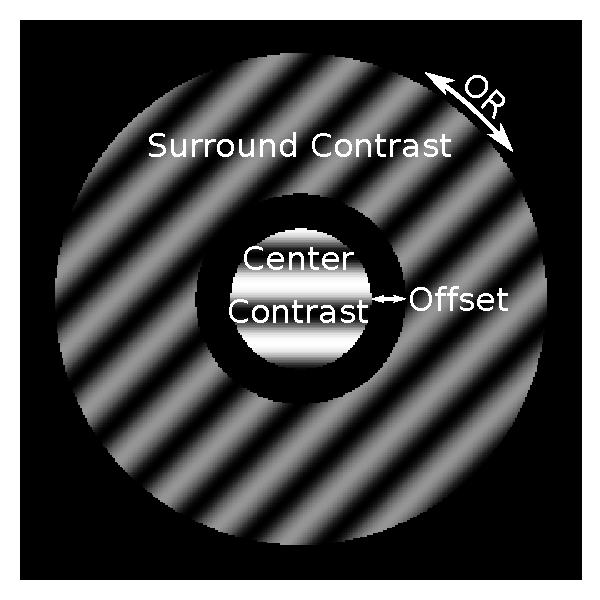
\includegraphics[width=0.5\textwidth]{ORC_Stimulus.pdf}
	\caption{Orientation contrast stimulus measuring modulation by a
      sine grating annulus on the response of a central neuron
      responding to a central sine grating disk of the same frequency.
      Stimulus is varied by center and surround contrast, surround
      orientation and the offset between the central disk and the
      surround annulus.}
	\label{ORC_Stimulus}
\end{figure}

The surround facilitation is quantified as:

\begin{equation}
F = (\frac{R_{cs}}{R_c} - 1) * 100
\end{equation}

where $R_{CS}$ is the response of the combined stimulus and $R_C$ the
response to just the center stimulus.

\paragraph{Flanker Modulation}

Instead of working solely using area based protocols we also make use
of a simple bar based stimulus along with a flanker, which is
modulated in a number of ways to characterize the surround modulation
effects associated with this protocol. In \cite{Kapadia1995} describe
a high degree of variability ranging from a complete lack of surround
modulation to facilitation and suppression. The three stimulus
protocols employed here are shown in \ref{Flanker}, we replicate these
protocol on the model to compare the effects observed in experiments
qualitatively.

\begin{figure}
	\centering
        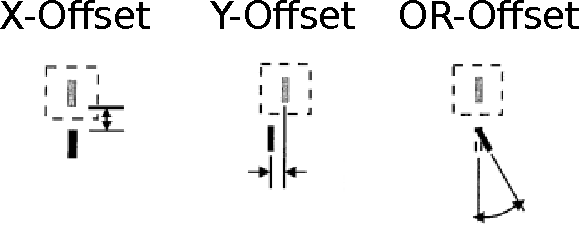
\includegraphics[width=1.0\textwidth]{FlankerProtocol.pdf}
	\caption{Flanker offset surround modulation paradigm. Measuring
      the effect of a flanker stimulus varying by an offset in X, Y
      and orientation on the response of a neuron to a target
      stimulus.}
	\label{Flanker}
\end{figure}

\section{Results}

A major component of the work in this chapter was optimizing for a
wide range of measures to achieve rough agreement with the wide range
of experimentally confirmed measurements

\subsection{Spatially calibrating LGN receptive fields}

In spatially calibrating the spatial properties of LGN receptive
fields we must take into account how they will contribute to the V1
receptive fields. One major issue in accurately modeling the LGN
connectivity is that no detailed anatomical measurements exist
describing the extent of LGN neurons and spatial measurements are
highly dependent on stimulus parameters.

In \ref{LGNTuning} we summarize population estimates from a number of
studies, measured by presenting disk masked sine gratings of varying
sizes and fitting the responses with a Difference of Gaussian model.
The estimates here vary widely with the results from
\citep{Sceniak2006} being the particular outlier. Another concern is
that it is not clear how these values translate into the existing LGN
model. To confirm this we will replicate the experimental protocols
used to obtain these values.

\begin{table}
  \centering
  \begin{adjustbox}{width=1\textwidth}
  \begin{tabular}{l | l l l l l l}
    Connection   & Literature            & Species  & Ecc. ($\degree$) & Model & Layer & $R_{c/s}$ \\
    \hline
    LGN Center   & \cite{Sceniak2006}    & macaque  & 2-5  & parvo & - & $median = 0.46 \degree$ $mean = 0.5 \degree$ \\
                 & \cite{Levitt2001}     & macaque  & 0-10 & parvo & - & $0.069 \pm 0.076 \degree$ \\
                 & \cite{Spear1994}      & macaque  & 0-10 & parvo & - & $0.087 \pm 0.046 \degree$ \\
                 & \cite{Bonin2005}      & macaque  & 13.9 & parvo & - & $0.6 \pm 0.4 \degree$\\
                 &                       &          &      &       & / & $0.4 \pm 0.2 \degree$ \\
    \hline
    LGN Surround & \cite{Sceniak2006}    & macaque  & 2-5  & parvo & - &$median = 0.51 \degree$ (0.15-0.85) \\
                 & \cite{Levitt2001}     & macaque  & 0-10 & parvo & - & $0.33 \pm 0.076 \degree$ \\
                 & \cite{Spear1994}      & macaque  & 0-10 & parvo & - & $0.53 \pm 0.39 \degree$ \\
                 & \cite{Bonin2005}      & macaque  & 13.9 & parvo & - & $2.0 \pm 1.1 \degree$\\
                 &                       &          &      &       & / & $1.8 \pm 2.6 \degree$\\

    \hline
  \end{tabular}
  \end{adjustbox}
  \caption{Estimates of LGN neuron spatial tuning properties fitted using Difference of Gaussian models
           with either subtractive or divisive suppressive components.}
  \label{LGNEstimates}
\end{table}

A set of area-summation curves measured at varying contrast levels can
be seen in Figure \ref{LGNSizeTuning}. These curves were then fitted
using the iDoG model resulting in the fit shown in Figure
\ref{LGNSizeFit}. Through an iterative process we could determine
establish a rough correspondence between the kernel sizes used in the
model definition and those obtained through the model fitting
process. However, in particular the surround size was consistently
overestimated using this procedure.

\begin{figure}
	\centering
        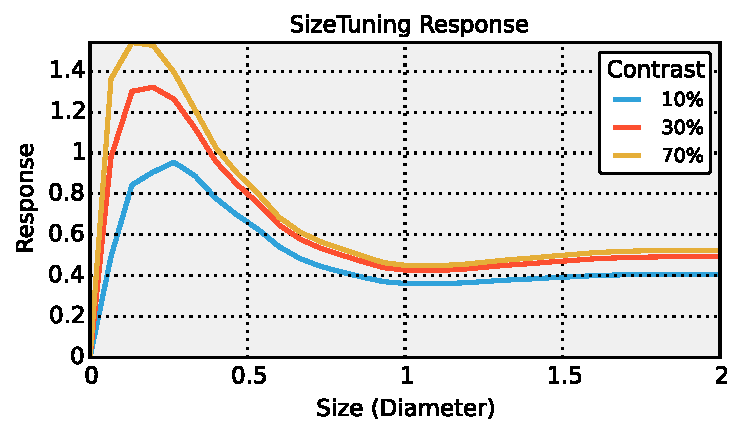
\includegraphics[width=1.0\textwidth]{LGN_SizeTuning.pdf}
	\caption{}
	\label{LGNSizeTuning}
\end{figure}

\begin{figure}
	\centering
        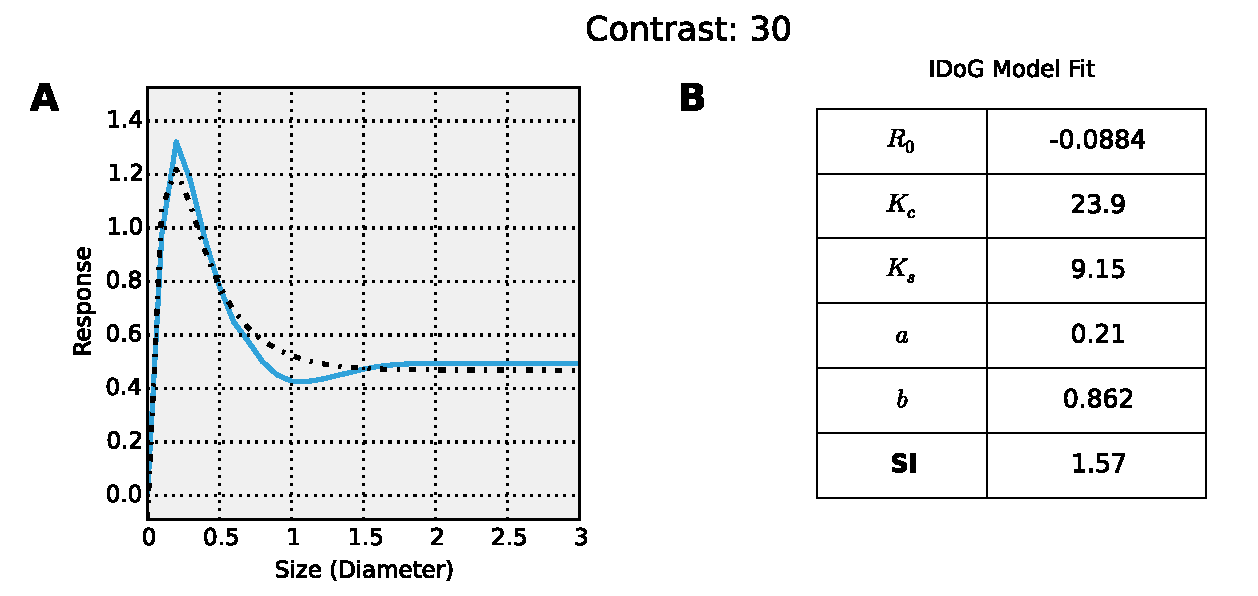
\includegraphics[width=1.0\textwidth]{LGN_SizeFit.pdf}
	\caption{A) LGN area-summation curve (blue) fit using an
          integrated Difference-of-gaussian model (dotted). B)
          Parameters of the iDoG model fit.}
	\label{LGNSizeFit}
\end{figure}

Note that neither of these models captures the mechanisms of the
SCAL-LGN model described above, which although it too operates on DoG
center-surround fields uses joint normalization and adds a distinct
divisive component, independent of the subtractive surround.

In the end it was decided that due to the large variance in results
from different studies and the limitation to a single spatial filter a
lower spatial constants should be chosen for the center-surround
mechanism. This choice allowed a fairly broad range of spatial
frequencies to be relayed to V1 to account for the lack of spatial
filter diversity. Future models should aim to cover the full
distribution of spatial frequency and size sensitivities. The final
model parameters are summarized in \ref{LGNTuning} and visualized in
Figure \ref{LGNDiagram}.
 
\begin{table}
  \centering
  \begin{adjustbox}{width=0.3\textwidth}
  \begin{tabular}{l | r}
    Model parameter   & Value \\
    \hline
    $\sigma_c$          & $0.1 \degree$  \\
    $\sigma_s$          & $0.15 \degree$ \\
    $\sigma_{gc}$        & $0.25 \degree$  \\
    $radius_{c+s}$       & $0.3 \degree$  \\
    $radius_{gc}$        & $0.5 \degree$  \\
    \hline
    $LGN_{aff}$ strength & 14 \\
    $LGN_{GC}$ strength  & 0.6 \\
  \end{tabular}
  \end{adjustbox}
  \caption{Parameters for S-patially CAL-ibrated (SCAL) LGN model.}
  \label{LGNTuning}
\end{table}

\subsection{Spatially calibrating V1 receptive fields}

A neuron in primary visual cortex receives input from a variety of
sources, including feedforward connections from the LGN, horizontal
connections from within V1 and feedback connections from extrastriate
cortex as seen in Figure \ref{Angelucci2006}. Achieving a consistent
spatial tuning is therefore a complex problems relying on a large
variety of measurements.

\begin{table}
\centering
\begin{tabular}{l | c c}
  \hline
  \hline
  Visual Area     & Magnification Factor ($mm/\deg$) & Anisotropy Index \\
  \hline
  Retina$^1$      & 0.223                            & -                      \\
  LGN$^2$         & 0.324                             & 1.0-2.0                \\
  V1$^3$          & 2.54-3.545                       & 1.0-3.0                \\
  \hline
\end{tabular}
\caption[]%
{Magnification Factors and Anisotropy Index associated with different visual areas at $3\degree$ eccentricity estimated from areal and linear magnification factor equations. Footnotes: $^1$ - \cite{Perry1985}, $^2$ - \cite{Connolly1984}, $^3$ - \cite{VanEssen1984}}
\label{MFs}
\end{table}

The first step towards a spatially calibrated model is to decide on
the region of V1 that should be targeted. Most studies of V1
particularly in the surround modulation literature focuss on parafoveal
regions between $2-5\degree$ in eccentricity. Therefore we have chosen
a region at around $3\degree$ eccentricity. This already gives us a
number of constraints, first of all gives us an approximate V1
magnification factor of 3 mm/deg as described by \cite{VanEssen1984}
and shown in Table \ref{MFs}.

Secondly to give actual scale to our model we can measure the
orientation map hypercolumn distance, which has been well established
in the literature. Using estimates provided by the Wolf group the
hypercolumn distance in macaque V1 has been estimated at roughly \(710
\pm 50 \mu m\). By combining this information with the magnification
factor we can establish that we'd expect roughly 4.2 hypercolumns per
visual degree and to keep things simple we will keep a 1:1 mapping
between visual angle and sheet coordinates of the model. We will also
define an acceptable range of hypercolumn cycles per degree to ensure
later models do not diverge too far from the spatial tuning
implemented here. Taking the confidence intervals for both the
magnification factor and hypercolumn distance into account the
acceptable range of hypercolumns per sheet coordinate is between 3.29
and 5.3.

\subsection{Methods}

The hypercolumn distance was calculated by taking the 2D Fourier
transform of the orientation map, reducing it to one dimension and
applying a least-squares fit of a Gaussian curve with additional
linear and quadratic terms (see \cite{Kaschube2010} for more
details). A sample fit to an SCAL orientation map can be seen in
Figure \ref{SCALhypercolumns}. The actual spatial calibration
procedure then was an iterative process between this hypercolumn fit
and ensuring that all the connectivity kernels matched the
experimental results outlined in the tables outlining both anatomical
results (\ref{anatomicaltable}) and electrophysiological measurements
(\ref{electrophystable}).

In particular we confirmed the spatial tuning of the afferents,
independently from the lateral connections. While electrophysiological
results were again fit using the DoG model and compared against
experimental results, the lateral connectivity was fit with a
descriptive model of the patchy, excitatory connectivity found in
layer 2/3 of the visual cortex and again compared against the
experimentally observed values.

\begin{table}
  \centering
  \begin{adjustbox}{width=1\textwidth}
  \begin{tabular}{l | l l l l}
    Connection               & Literature            & Species & Layer & $\sigma$ \\
    \hline
    LGN-V1 Afferents         & \cite{Angelucci2002c} & macaque & 4C$\alpha$ & $0.8-1.6\degree$ \\
                             & \cite{Angelucci2006a} & macaque & 4A/4C$\beta$ & $0.91 \pm 0.041 \degree$ \\
    \hline
    V1 local excitation      & \cite{Buzas2006}      & cat      & 2-4 single cell & $288 \mu m$ \\
                             & \cite{Buzas2006}      & cat      & 2-4 population  & $520 \mu m$ \\
    \hline
    V1 basket cells          & \cite{Buzas2001}      & cat      & 2-6 & $0.7-1.9 \degree$ \\
                             & \cite{Buzas2001}      & cat      & 2-6 & $0.76-2.6 mm$ \\
    \hline
    V1 long-range excitation & \cite{Angelucci2002}  & macaque  & 2/3 & $6\pm 0.7 mm$ (3-9) \\
                             &                       &          & 4B/4C$\alpha$ & $6.7 \pm 0.7 mm$ (4.7-10) \\
                             &                       &          & population & $2.47 \pm 0.3 \degree$ \\
                             & \cite{Buzas2006}      & cat      & 2/3 & $6 mm$ \\
    \hline
  \end{tabular}
  \end{adjustbox}
  \caption[]%
          {Anatomical estimates of the spatial profiles of V1 connectivity.}
  \label{anatomicaltable}
\end{table}

\begin{table}
  \centering
  \begin{adjustbox}{width=1\textwidth}
  \begin{tabular}{l | l l l l}
    Measurement              & Literature            & Species & Layer & $\sigma$ \\
    \hline
    V1 hsRF                  & \cite{Levitt2002}     & macaque & 2-6 & $1.0 \pm 0.2 \degree$ (0.3 - 2.2) \\
    \hline
    V1 Excitatory DoG fit    & \cite{Levitt2002}     & macaque & 2-6 & $0.9 \degree$ \\
                             & \cite{Sceniak2001}    & cat     & 2-6 & $1.0 \degree$ \\
                             & \cite{Cavanaugh2002}  & macaque & 2-6 & $1.4 \degree$ \\
                             & \cite{Solomon2002}    & macaque & not stated & $0.94 \degree$ \\
    \hline
    V1 Inhibitory DoG fit    & \cite{Levitt2002}     & macaque & 2-6 & $1.9 \degree$ \\
                             & \cite{Sceniak2001}    & cat     & 2-6 & $2.2 \degree$ \\
                             & \cite{Cavanaugh2002}  & macaque & 2-6 & $2.7 \degree$ \\
                             & \cite{Solomon2002}    & macaque & not stated & $2.97 \degree$ \\
    \hline
  \end{tabular}
  \end{adjustbox}
  \caption[]%
          {Functional estimates of V1 receptive field size using Difference-of-Gaussian models.}
  \label{electrophystable}
\end{table}

\begin{figure}
	\centering
        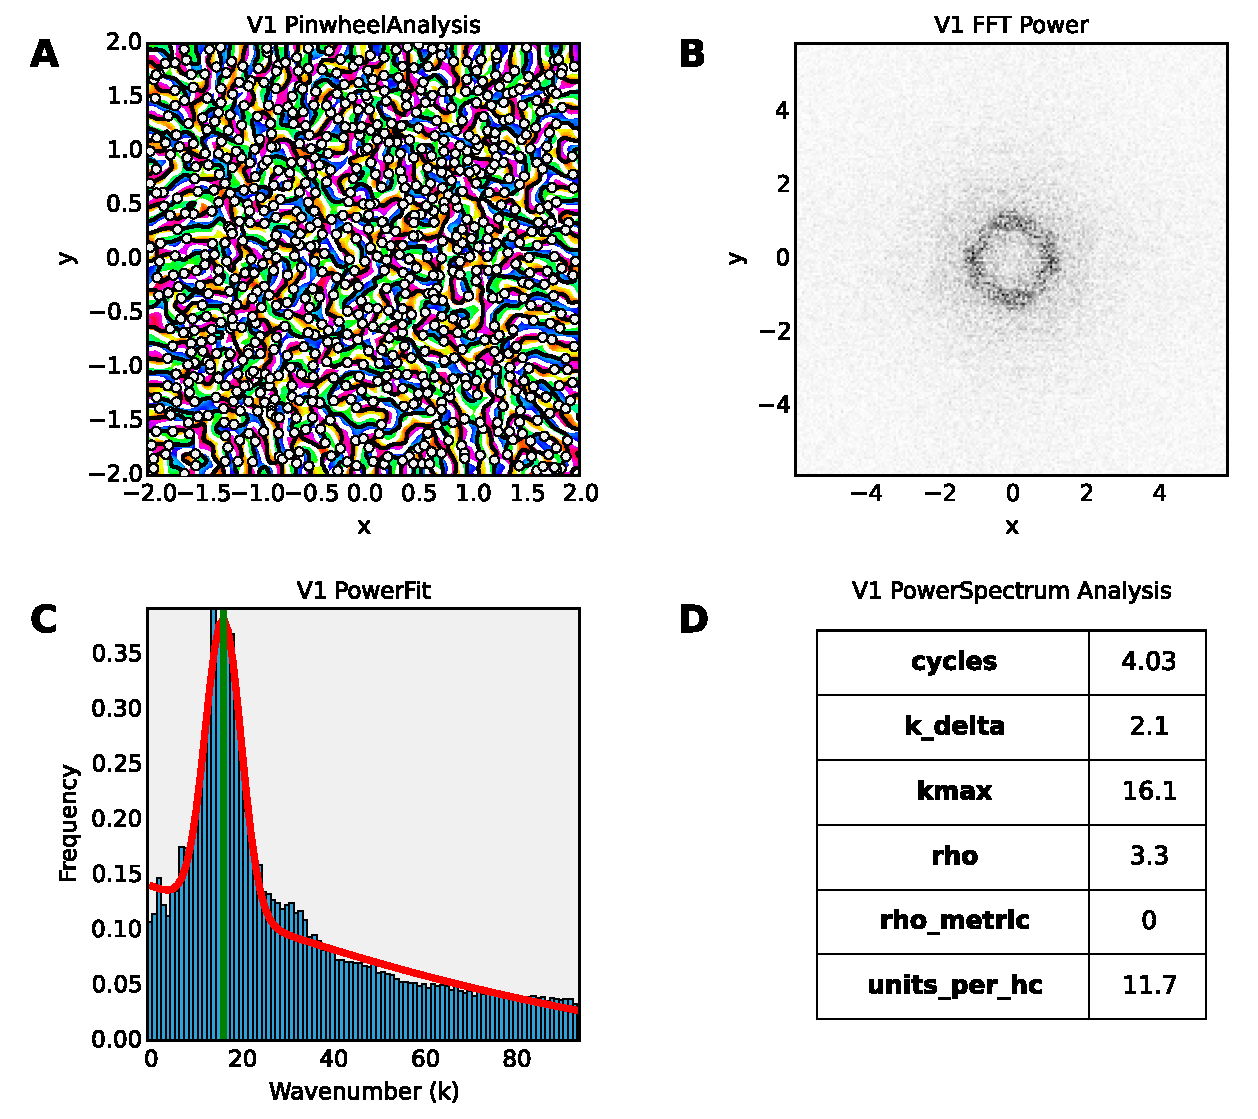
\includegraphics[width=1.0\textwidth]{SCAL_hypercolumns.pdf}
	\caption{Hypercolumn and pinwheel density fitting
          procedure. A) Orientation map in V1 overlaid with real and
          imaginary contours and pinwheels at their intersections. B)
          2D FFT of the orientation map showing a ring identifying the
          periodicity of the map. C) 1D histogram of the FFT along
          with Gaussian fit marking the best fit hypercolumn distance.
          D) Summary table showing various parameters of the fit,
          along with pinwheel density ($\rho$) which classifies the
          quality of the map.}
	\label{SCALhypercolumns}
\end{figure}

\subsection{Feedforward}

The first step in the fitting procedure was to repeat the protocols
applied to the LGN, i.e. measuring area summation curves and fitting
DoG models to the results. Using this approach we obtained a large
number of size estimates for the excitatory and inhibitory kernels
contributing to the V1 response.

\begin{figure}
	\centering
        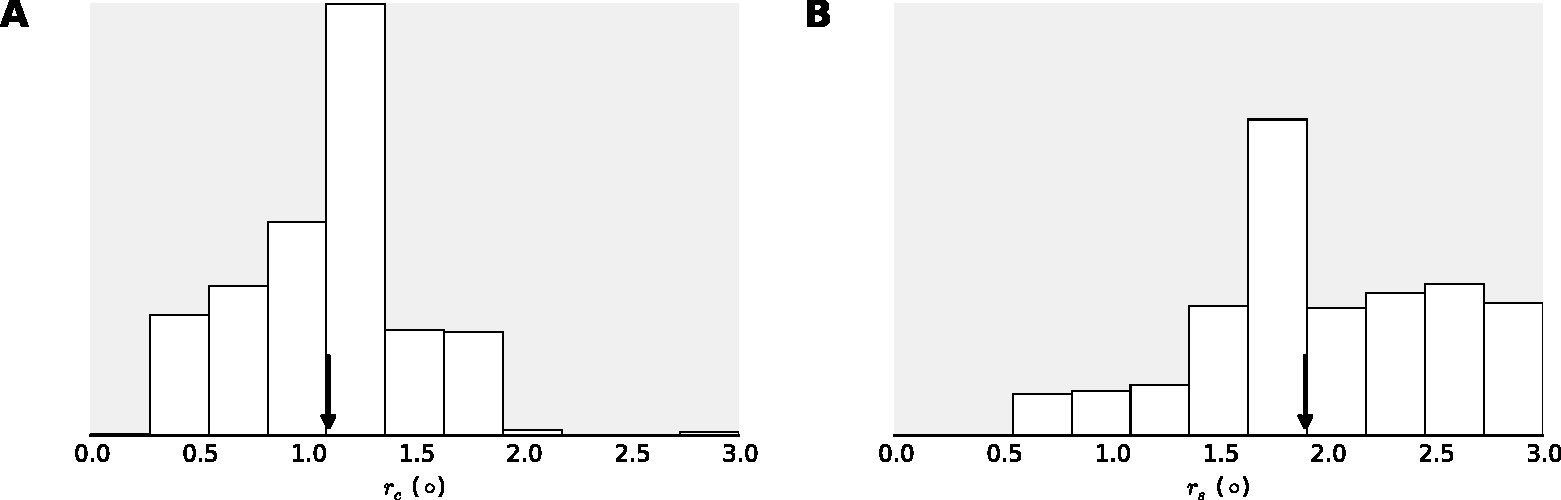
\includegraphics[width=1.0\textwidth]{SCAL_SizeDist.pdf}
	\caption{Distribution of excitatory (A) and inhibitory (B)
          Difference-of-Gaussian components fitted to area-summation
          curves measured in the SCAL V1 model. These results provide
          a close match to the results seen in Fig. 12 \& 14 of
          \cite{Sceniak2001}.}
	\label{SCALSizeDist}
\end{figure}

\subsubsection{Area summation}

Summarize table and electrophysiological results
Replicate area summation procedure
Compare distributions of fits

\subsection{Receptive Fields}

* Discuss Ringach nx/ny ratios
* Plot nx/ny plot, with overlaid fit
* Discuss circular CFs and limited filters



\subsection{Intracortical connectivity}

The intracortical connectivity can be further divided into excitatory
and inhibitory populations, we will outline the protocols for tuning
each.

\subsubsection{Excitatory Connections}

The literature has had a much harder time of picking apart the
contribution of intracortical and particularly the patchy lateral
connectivity found in V1 so to confirm that these connections have
developed as expected is to compare it to anatomical measurements.
For this purpose we will be fitting a descriptive model, developed by
\cite{Buzas2006} to the lateral connectivity data.

\begin{figure}
	\centering
        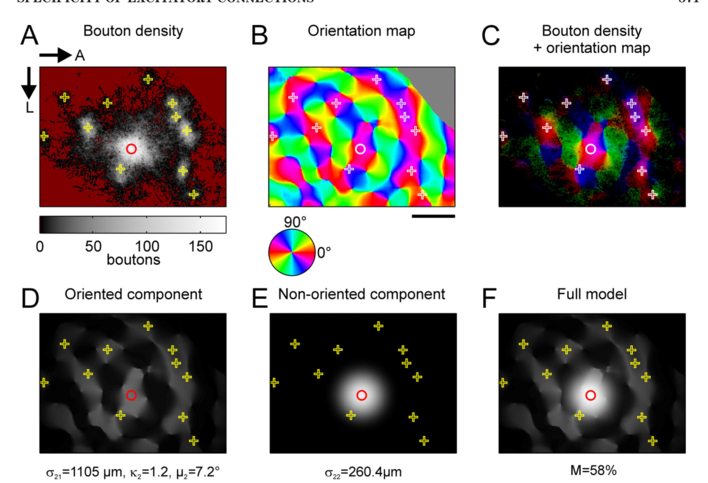
\includegraphics[width=1.0\textwidth]{Buzas.png}
	\caption{Lateral excitatory projection bouton density and
          orientation maps in layer 2/3 of cat V1 fit using a Gaussian
          and vonMises model, replicated from \cite{Buzas2006}.}
	\label{Buzas}
\end{figure}

The model describes the patchy lateral connectivity found in layer 2/3
of V1 as a function of two distinct components. A short range
isotropic Gaussian pattern and a long range pattern, defined as a von
Mises function, which is combined with the orientation map. The model
therefore assumes that lateral connectivity develops as a function of
both the proximity in space but also along a particular feature
dimension, in this case the orientation.


The full model fitting procedure for an experimentally traced lateral
connection field is shown in Figure \ref{Buzas}. By applying this
fitting procedure we can effectively estimate the spatial extents of
both the local isotropic local kernel and the long-range excitatory
kernel. In Figure \ref{SCAL_Laterals.pdf} demonstrates what one such
fit looks like for the SCAL model, while the full distribution of
local and long-range kernel values is shown in \ref{LatDist}.

The distance of long-range connectivity varies even more considerably
across species so using some anatomical estimates from macaque we will
attempt to refine our estimates of the long-range oriented
component. Anatomic data suggests that the spatial spread of lateral
connections can be anywhere between 3-10 mm (on average 6-7 mm) in
total length \cite{Angelucci2002}. Along its principal axis the
visuotopic monosynaptic spread of V1 horizontal connections has a mean
of \(2.47^\circ\) \(\pm\) \(0.3^\circ\). This falls well within the
range of estimates for the lsRF as published in a number of studies
\cite{Sceniak1999, Sceniak2001, Shushruth2009}, which employed the
iDoG protocol.

The results of our fitting procedure shown in Figure \ref{LatDist}
show good correspondence with these experimental estimates with a mean
long-range connectivity that has a spatial constant of around 5 mm but
extends beyond that with our cut-off defined at $2.5\degree$ or $7.5
mm$. The local excitatory kernel also matches experimental estimates
closely with a mean local excitatory kernel with a spatial constant of
around $350 \mu m$, compared to the $280 \mu m$ estimated in cat V1.

\begin{figure}
	\centering
        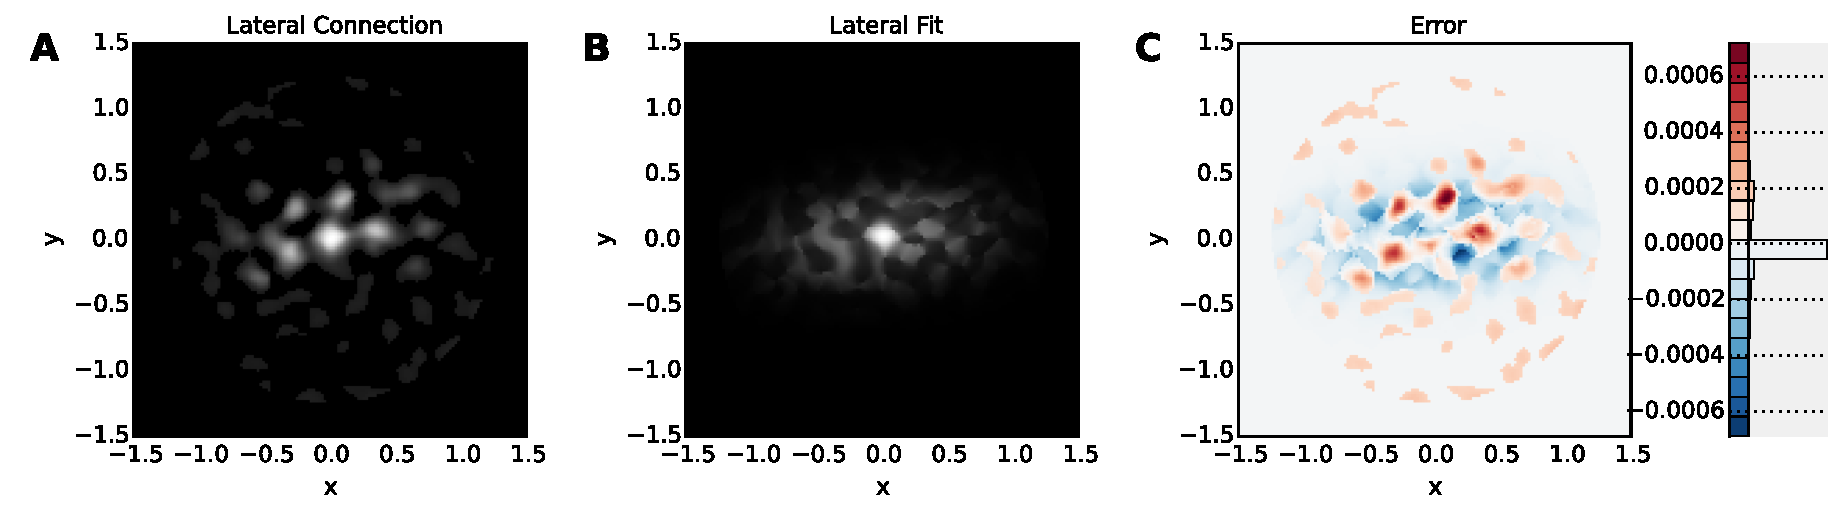
\includegraphics[width=1.0\textwidth]{SCAL_Laterals.pdf}
	\caption{Distribution of spatial constant obtained by fitting
          the \cite{Buzas2006} vonMises+Gaussian model to long-range
          lateral excitatory connections developed as part of the SCAL
          model.}
	\label{LatFits}
\end{figure}

\begin{figure}
	\centering
        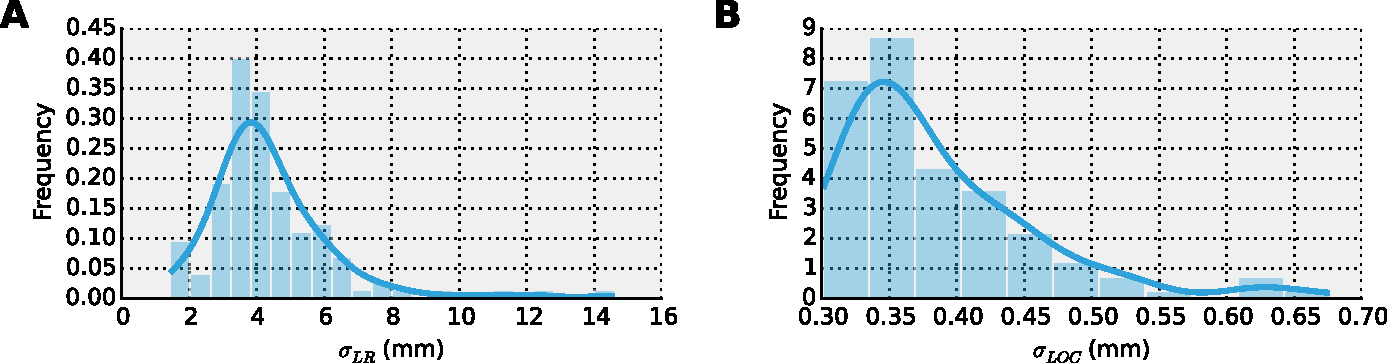
\includegraphics[width=1.0\textwidth]{SCAL_LateralFits.pdf}
	\caption{Distribution of spatial constant obtained by fitting
          the \cite{Buzas2006} vonMises+Gaussian model to long-range
          lateral excitatory connections developed as part of the SCAL
          model.}
	\label{LatDist}
\end{figure}

\subsection{Inhibitory connectivity}

The literature surrounding inhibitory connectivity is much more
limited and no good estimates of cell-type specific spatial profiles
particularly for the primate visual cortex exist. Therefore we have to
extrapolate from existing data. In the literature review we explored
the known properties of various cell classes and identified
fast-spiking Parvalbumin-expressing interneurons as the most likely
source of connectivity to drive developmental, particularly due to
their broad tuning profile and high abundance in the thalamocortical
recipient layers. Since the SCAL model does not have distinct
populations of V1 we will consider the maximal extent of known basket
cells as the maximal permitted extent of the inhibitory profile in the
model. We will revisit the spatial profiles of inhibitory connections
in the next chapter.

\subsection{Sparse connectivity}

* Real neurons only receive a few number of afferents (citation)
* We can develop sparse connectivity profiles
* Map quality does not suffer
* Show figure


\section{Conclusions}

\begin{figure}
	\centering
        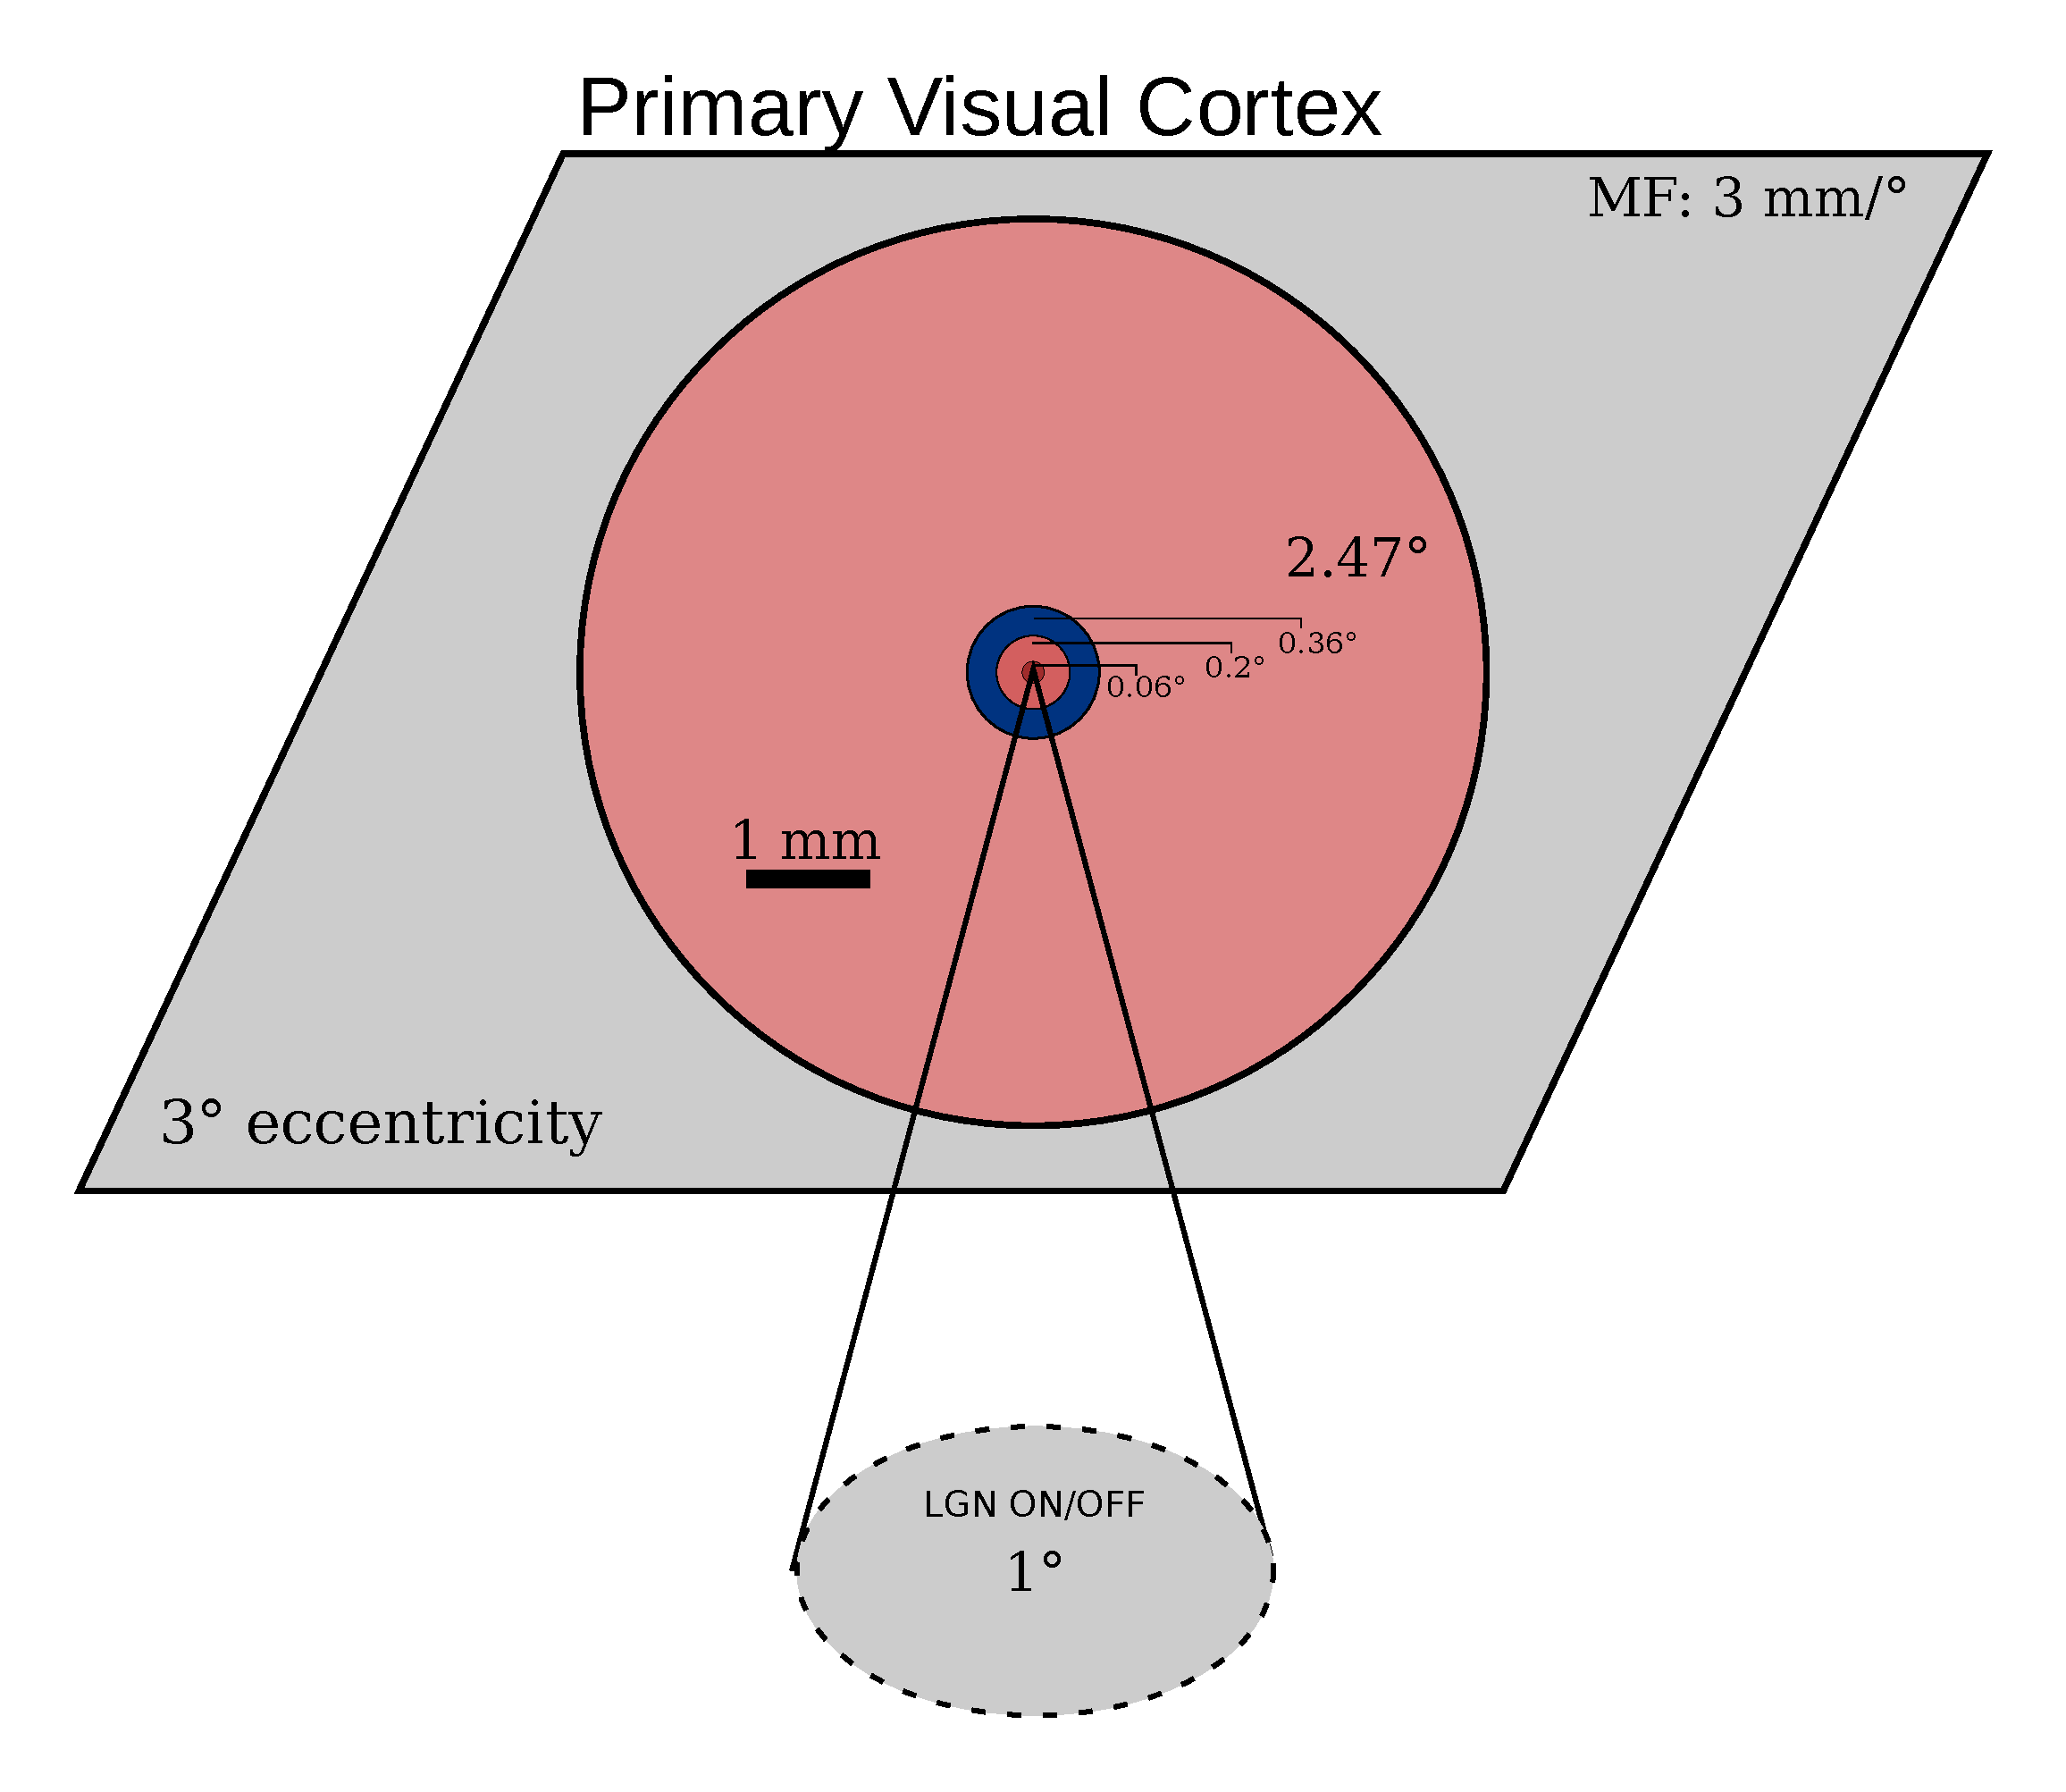
\includegraphics[width=1.0\textwidth]{SCAL_Diagram.pdf}
	\caption{Diagram of the SCAL V1 stage of the model showing
          the spatial scales of the various excitatory (red) and
          inhibitory (blue) connections. Satured colors indicate the
          kernel radii, while lightly shaded regions indicate kernel
          cut-off extents.}
	\label{SCALDiagram}
\end{figure}


To be done:

\begin{itemize}
  \item Add further plots describing the size and frequency tuning of SCAL V1.
  \item Provide further details on the lateral connectivity model fits and suggest extension based on selectivity.
  \item Optionally add analysis showing that RF nx/ny ratios closely
    follow Ringach results.
  \item Potentially add section that shows that the model can develop with realistic numbers of afferents (~30) and that lateral connectivity can be hugely sparsified (over 90\%) with little effect.
\end{itemize}
